\documentclass{article}
\begin{enumerate}
\item
Draw a game tree for the first two moves (\texttt{A} moves
then \texttt{B} moves.
\marginpar{[10 pts]}
This tree should show the actual board setups!
\textbf{Solution:}
\begin{minipage}[t][5cm][t]{0.9\textwidth}

\begin{center}
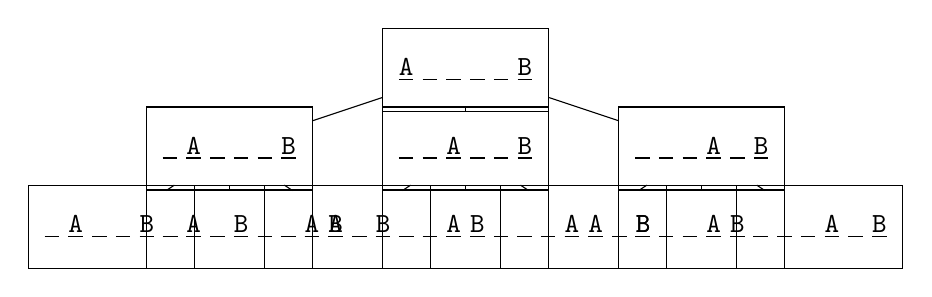
\begin{tikzpicture}[scale=0.5]
\tikzstyle{vertex}=[rectangle, minimum width=60pt, minimum height=30pt, inner sep=2pt, draw=black]

% Root node
\node[vertex] (v0) at (0,0) {\underline{\texttt{A}}
\underline{\texttt{ }}
\underline{\texttt{ }}
\underline{\texttt{ }}
\underline{\texttt{ }}
\underline{\texttt{B}}};

% A's possible moves
\node[vertex] (v1) at (-6,-2) {\underline{\texttt{ }}
\underline{\texttt{A}}
\underline{\texttt{ }}
\underline{\texttt{ }}
\underline{\texttt{ }}
\underline{\texttt{B}}};
\node[vertex] (v2) at (0,-2) {\underline{\texttt{ }}
\underline{\texttt{ }}
\underline{\texttt{A}}
\underline{\texttt{ }}
\underline{\texttt{ }}
\underline{\texttt{B}}};
\node[vertex] (v3) at (6,-2) {\underline{\texttt{ }}
\underline{\texttt{ }}
\underline{\texttt{ }}
\underline{\texttt{A}}
\underline{\texttt{ }}
\underline{\texttt{B}}};

% B's possible moves from v1
\node[vertex] (v4) at (-9,-4) {\underline{\texttt{ }}
\underline{\texttt{A}}
\underline{\texttt{ }}
\underline{\texttt{ }}
\underline{\texttt{B}}
\underline{\texttt{ }}};
\node[vertex] (v5) at (-6,-4) {\underline{\texttt{ }}
\underline{\texttt{A}}
\underline{\texttt{ }}
\underline{\texttt{B}}
\underline{\texttt{ }}
\underline{\texttt{ }}};
\node[vertex] (v6) at (-3,-4) {\underline{\texttt{ }}
\underline{\texttt{A}}
\underline{\texttt{B}}
\underline{\texttt{ }}
\underline{\texttt{ }}
\underline{\texttt{ }}};

% B's possible moves from v2
\node[vertex] (v7) at (-3,-4) {\underline{\texttt{ }}
\underline{\texttt{ }}
\underline{\texttt{A}}
\underline{\texttt{ }}
\underline{\texttt{B}}
\underline{\texttt{ }}};
\node[vertex] (v8) at (0,-4) {\underline{\texttt{ }}
\underline{\texttt{ }}
\underline{\texttt{A}}
\underline{\texttt{B}}
\underline{\texttt{ }}
\underline{\texttt{ }}};
\node[vertex] (v9) at (3,-4) {\underline{\texttt{ }}
\underline{\texttt{ }}
\underline{\texttt{A}}
\underline{\texttt{ }}
\underline{\texttt{ }}
\underline{\texttt{B}}};

% B's possible moves from v3
\node[vertex] (v10) at (3,-4) {\underline{\texttt{ }}
\underline{\texttt{ }}
\underline{\texttt{ }}
\underline{\texttt{A}}
\underline{\texttt{ }}
\underline{\texttt{B}}};
\node[vertex] (v11) at (6,-4) {\underline{\texttt{ }}
\underline{\texttt{ }}
\underline{\texttt{ }}
\underline{\texttt{A}}
\underline{\texttt{B}}
\underline{\texttt{ }}};
\node[vertex] (v12) at (9,-4) {\underline{\texttt{ }}
\underline{\texttt{ }}
\underline{\texttt{ }}
\underline{\texttt{A}}
\underline{\texttt{ }}
\underline{\texttt{B}}};

% Connect nodes
\draw (v0) -- (v1);
\draw (v0) -- (v2);
\draw (v0) -- (v3);

\draw (v1) -- (v4);
\draw (v1) -- (v5);
\draw (v1) -- (v6);

\draw (v2) -- (v7);
\draw (v2) -- (v8);
\draw (v2) -- (v9);

\draw (v3) -- (v10);
\draw (v3) -- (v11);
\draw (v3) -- (v12);
\end{tikzpicture}
\end{center}

\end{minipage}
\item
Draw a second tree which contains the heuristic values for the leaves
\marginpar{[10 pts]}
and then fill in the remaining values according to the Minimax algorithm.
\textbf{Solution:}
\end{enumerate}
\end{enumerate}
\end{document}